\scanpage{29}
\mspage{15}
\textcircled{9} \uline{An arithmetico-geometric} \uline{conjecture}

Let $g,\nu\geq0$ be integers. We denote by $\deleted{\unsure{\mathcal T}}M_{g,\nu}$ the modular topos 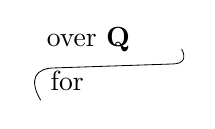
\begin{tikzpicture}[baseline=(base.base)]
\node[anchor=base west,inner sep=0] (base) at (0,0) {for};
\node[anchor=base west,inner sep=0] at (-0.05,.56) {\inserted{over $\mathbf Q$}};
\draw[line width=.3pt] (-.12,-.12) .. controls (-.28,.15) and (-.18,.29) .. (.06,.29) -- (1.55,.34) .. controls (1.7,.34) and (1.73,.42) .. (1.67,.53);
\end{tikzpicture} the 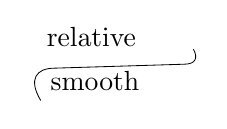
\begin{tikzpicture}[baseline=(base.base)]
\node[anchor=base west,inner sep=0] (base) at (0,0) {smooth};
\node[anchor=base west,inner sep=0] at (-0.05,.56) {\inserted{relative}};
\draw[line width=.3pt] (-.12,-.12) .. controls (-.28,.15) and (-.18,.29) .. (.06,.29) -- (1.7,.34) .. controls (1.8499999999999999,.34) and (1.88,.42) .. (1.8199999999999998,.53);
\end{tikzpicture} proper relatively connected curves of genus $g$, \uline{equipped} with \deleted{\unsure{a}} $\nu$-tuple of $\nu$ sections disjoint on each fiber

Except for $g=0$, $\nu=0,1,2$ and $g=1$, $\nu=0$, this topos is associated \unsure{to|:} an algebraic étendue, related notion = \unsure{schemable}.

We have a natural \deleted{\unsure{outer}} homomorphism
\[
\pi_1(\deleted{\unsure{\mathcal T}}M_{g,\nu};\xi)\longrightarrow\operatorname{Autextlac}^{\circ}\bigl(\pi_1(\overline X\setminus\{x_1,\mathbin{-},x_\nu\})\bigr)\tag{1}
\]
where $(X;x_1,\mathbin{-}x_\nu)$ $\longrightarrow$ the corresponding point 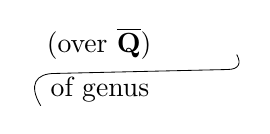
\begin{tikzpicture}[baseline=(base.base)]
\node[anchor=base west,inner sep=0] (base) at (0,0) {of genus};
\node[anchor=base west,inner sep=0] at (-0.05,.56) {\inserted{(over $\overline{\mathbf Q}$)}};
\draw[line width=.3pt] (-.12,-.12) .. controls (-.28,.15) and (-.18,.29) .. (.06,.29) -- (2.25,.34) .. controls (2.4,.34) and (2.43,.42) .. (2.37,.53);
\end{tikzpicture} $\unsure{g|0}$ with $\nu$ marked points associated with $\xi$ 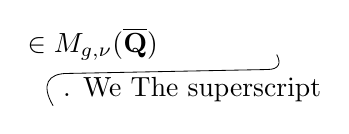
\begin{tikzpicture}[baseline=(base.base)]
\node[anchor=base west,inner sep=0] (base) at (0,0) {. \deleted{We} The superscript};
\node[anchor=base west,inner sep=0] at (-0.45,.56) {\inserted{$\in M_{g,\nu}(\overline{\mathbf Q})$}};
\draw[line width=.3pt] (-.12,-.12) .. controls (-.28,.15) and (-.18,.29) .. (.06,.29) -- (2.6,.34) .. controls (2.75,.34) and (2.7800000000000002,.42) .. (2.72,.53);
\end{tikzpicture} $\circ$ marks the fact that we take the automorphisms of $\pi_1$ which do not interchange among themselves the classes of loops associated with the $x_i$\unsure{--|.}
\margin{perhaps one must be stricter, and require commutation : of the defined actions : of $\mathfrak S_\nu$ on the $\pi_1$ ?? One must look especially at the case $g=0,\nu=3$....}

Note that we also have
\[
\pi_1(\overline M_{g,\nu};\xi)\longrightarrow\operatorname{Autextlac}^{\circ\circ}\bigl(\pi_1(X\setminus\{x_1,\mathbin{-}x_\nu\})\bigr)\tag{2}
\]
where the double $\circ$ indicates that we take \inserted{\uline{strict}} automorphisms compatible with the structure : \unsure{local|loops}, \unsure{(i.e.|i.e.} inducing the identity on $T=\operatorname{Tate}(\overline{\mathbf Q})$\ldots
\margin{\unsure{Oriented} automorphisms}
\[
\pi_1(M_{g,\nu}^{an};\xi)\longrightarrow
\mathrm{Aut}\underbrace{\mathrm{extlac}^{\circ\circ}\pi_1(X^{an}\setminus\{}_{\overset{\unsure{\deleted{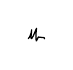
\begin{tikzpicture}[baseline=0pt,x=.45em,y=.4em,line width=.45pt,line cap=round,line join=round]\draw (0,.12) .. controls (.08,.18) and (.25,.56) .. (.27,.91) -- (.21,.19) .. controls (.19,.02) and (.33,.11) .. (.39,.34) -- (.66,1.05) .. controls (.62,.70) and (.58,.16) .. (.64,-.08) .. controls (.66,-.14) and (.76,.18) .. (.80,.26) -- (1.28,.20) -- (1.30,.10);\end{tikzpicture}}}}{=}\mathcal T_{g,\nu}\ (\text{Teichmüller})}x_1,\mathbin{-}x_\nu\})\tag{2 bis}
\]
which we know (topological theory) is a
\mspage{28}
